\documentclass[aspectratio=169]{beamer}
\usepackage{graphics,amssymb,amsfonts,amsmath}
\usepackage{tikz}
\DeclareGraphicsExtensions{.jpg,.pdf,.mps,.png}
\usepackage[latin1]{inputenc}
\usepackage[brazil]{babel}
\usepackage[normalem]{ulem}
\usepackage{pgfpages,enumerate,hyperref}
\usepackage{palatino}   %Fonte sem serifa.
\usepackage{ragged2e}   %Par�grafo justificado.
\usetheme{AnnArbor}     %Alguns temas aceitam se��o, outros n�o.
\usecolortheme{orchid}
\usefonttheme[onlymath]{serif}
%\usetheme{CambridgeUS}
%\usetheme{Berkeley}
%\usetheme{Madrid}
%\usecolortheme{dolphin}
%\usetheme{Malmoe}
%\usecolortheme{lily}
%\usecolortheme{whale}

%colocando n�mero de p�ginas no slide.
\setbeamertemplate{footline}[frame number]

% desativando os botoes de navegacao.
\beamertemplatenavigationsymbolsempty

%Tela cheia
\hypersetup{pdfpagemode=FullScreen}

% Layout da p�gina: Duas colunas.
\hypersetup{pdfpagelayout=SinglePage}

%Defini��o de novos ambientes.
\theoremstyle{Definition}
\newtheorem{defn}{Defini��o}
\newtheorem{teo}[theorem]{Teorema}
\newtheorem{ex}[theorem]{Exemplo}

%Defini��o de novos comandos.
\providecommand{\sin}{} \renewcommand{\sin}{\hspace{2pt}\textrm{sen}}
\providecommand{\tan}{} \renewcommand{\tan}{\hspace{2pt}\textrm{tg}}
\newcommand{\R}{\mathbb{R}}

\title[\sc{Texto no rodap�}]{Modelo do Beamer Wide Screen}
\author[R�gis da Silva Santos]{R�gis da Silva Santos}
\institute{UFMT}
\date{\today}

\begin{document}
\justifying %Par�grafo justificado.

\begin{frame}
%Tela de apresenta��o com plano de fundo personalizado.
\begin{tikzpicture}[remember picture,overlay]
    \node at (current page.south west)
      {\begin{tikzpicture}[remember picture, overlay]
        \fill[shading=radial,top color=orange,bottom color=orange,middle color=yellow]
          (0,0) rectangle (\paperwidth,\paperheight);
      \end{tikzpicture}
      };
\end{tikzpicture}
\titlepage
\end{frame}

%Neste caso insere somente no primeiro slide.
{%
%\usebackgroundtemplate{\centering 
\includegraphics[width=\paperwidth]{figBackground}}

%Centralizado
\usebackgroundtemplate{%
\vbox to \paperheight{\vfil\hbox to \paperwidth{\hfil\includegraphics[width=\paperwidth]{figuras/djangoPython}\hfil}\vfil}
}

  \begin{frame}

    \begin{center}
      \Huge{Figura como plano de fundo}
    \end{center}
  \end{frame}
}

\begin{frame}[fragile]\frametitle{Express�es Matem�ticas}

%Paragrafo.
\setlength{\parindent}{2em}

Seja $f:\R \to \R$ tal que $y=\sqrt{x}$.

Este texto est� justificado \footnote{Nota de rodap�.} e com uma margem definida pelo comando

\begin{verbatim}
\setlength{\parindent}{2em}
\end{verbatim}

Exemplo de uma equa��o matem�tica centralizada.

\[
\sin^2 x + \cos^2 x = 1
\]

\end{frame}

\begin{frame}\frametitle{Links}

\begin{center}
www.google.com
\end{center}


\end{frame}

\begin{frame}[fragile]{Exemplo e c�digo}
\begin{block}{Exemplo}
Texto
\end{block}

\begin{exampleblock}{Solu��o}

\begin{verbatim}
\documentclass{beamer}
\usepackage{graphics,amssymb,amsfonts,amsmath}
\DeclareGraphicsExtensions{.jpg,.pdf,.mps,.png}
\usepackage[latin1]{inputenc}
\usepackage[brazil]{babel}
\usepackage[normalem]{ulem}
\usepackage{pgfpages,enumerate,hyperref,tikz}
\usepackage{palatino}   %Fonte sem serifa.
\usepackage{ragged2e}   %Par�grafo justificado.
\end{verbatim}

\end{exampleblock}
\end{frame}

\begin{frame}\frametitle{Novos ambientes}
\begin{defn}
Novo ambiente de defini��o.
\end{defn}

\begin{teo}
Novo ambiente de teorema.
\end{teo}
\end{frame}


\begin{frame}\frametitle{Inserindo figuras}

Figuras devem ser inseridas no formato PNG ou PDF.

\begin{figure}[h]
  \centering
  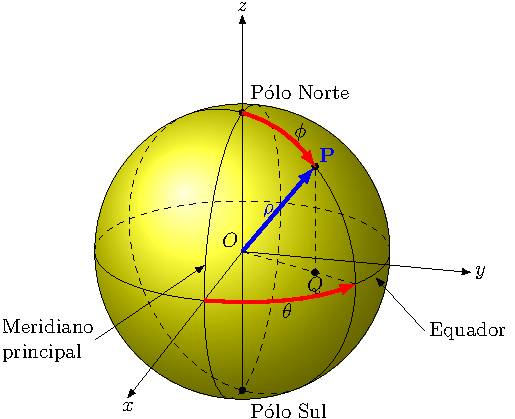
\includegraphics[height=0.6\paperheight]{figCoordEsf02}
  %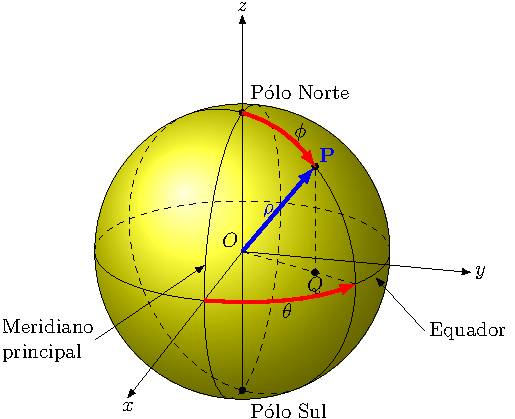
\includegraphics[height=6cm]{figCoordEsf02}
  \caption{Sistema de coordenadas esf�ricas.}\label{figCoordEsf02}
\end{figure}
\end{frame}

\begin{frame}\frametitle{Transi��es}

Texto ap�s uma pausa.

\pause

\begin{enumerate}[a)]
  \item<2-> primeiro;
  \item<3-> segundo;
  \item<4-> terceiro.
\end{enumerate}

\end{frame}

% Referencias bibliograficas
\begin{frame}\frametitle{Bibliografia}
\begin{thebibliography}{99}

\bibitem{Guidorizzi} GUIDORIZZI, Hamilton Luiz. {\sl Um Curso de C�lculo.} Vol. 1 e 2. 5� ed. Rio de Janeiro: LTC, 2007.

\bibitem{stewart} STEWART, James. {\sl C�lculo.} Vol. 1. 5� Ed. S�o Paulo: Pioneira, 2006.

\bibitem{Munem} MUNEM, Mustafa A. e FOULIS, David J. {\sl C�lculo.} Vol. 1 e 2. Rio de Janeiro: LTC, 1982.

\bibitem{leithold} LEITHOLD, D. Louis. {\sl O C�lculo com Geometria Anal�tica.} Vol. 1. S�o Paulo: Harbra, 1977.

\bibitem{kaplan} KAPLAN, Wilfred. {\sl C�lculo Avan�ado.} Vol. 1. S�o Paulo: Edgard Bl�cher, 1972.

\end{thebibliography}
\end{frame}

\end{document} 